% -*- TeX-engine: luatex -*-
\documentclass[dvipsnames,presentation,aspectratio=169,14pt]{beamer}
\usepackage{hastingstheme}
\usepackage{qrcode}
\titlegraphic{
\includegraphics[scale=.35]{static_figures/du_bn.pdf}}
\author{\large Massimiliano Fasi}
\date{}

% \usepackage{template}
% \renewcommand{\authorname}{Lawrence Mitchell\inst{*}}
\renewcommand{\authoremail}{\inst{*}\texttt{lawrence.mitchell@durham.ac.uk}}

% \renewcommand{\sessionnumber}{2}
% \renewcommand{\sessiontitle}{Memory hierarchy}


\usetikzlibrary{matrix,fit,positioning,calc}
\usepackage{pgfplots}
\usetikzlibrary{pgfplots.groupplots}
% \pgfplotsset{compat=1.15}
\usepackage{pgfplotstable}
% \date{}


\begin{document}

\title{\firasemibold\color{White}%
  {\fontsize{20}{0}\selectfont SESSION 2\\
    \fontsize{40}{40}\selectfont Memory\\hierarchy\par}}
\titleslide

\begin{frame}
  \frametitle{Sum reduction benchmark (Exercise 1)}
  \begin{columns}[c]
    \begin{column}{0.27\textwidth}
      \small
      \vskip -50pt
      \begin{itemize}[itemsep=5pt,wide=0pt]
      \item SIMD: 4 plateaus
      \item scalar: 3 plateaus
      \end{itemize}
    \end{column}
    \begin{column}{0.7\textwidth}
      \begin{center}
        \vskip -10pt
        \begin{tikzpicture}
          \begin{axis}[
            height=7cm,
            width=10cm,
            xlabel={Array size},
            ylabel near ticks,
            ylabel={MFlops/s},
            xmode=log,
            xtick={1,16,256,4096,65536,1048576},
            xticklabels={1kB,16kB,256kB,4MB,64MB,1GB},
            log basis x={10},
            style={font=\small},
            legend pos={north east},
            thick,
            legend style={
              cells={anchor=west, align=left},
              fill=bgcolor, font=\footnotesize}
            ]
            \pgfplotstableread[row sep=\\]{%
              kB scalar avx\\
              1 4735.04 25689.32\\
              2 4580.04 35475.57\\
              4 4504.35 40751.21\\
              8 4468.90 37854.32\\
              16 4453.18 36623.58\\
              32 4435.81 34807.33\\
              64 4304.03 25788.06\\
              128 4428.43 26194.16\\
              256 4230.27 26289.56\\
              512 4413.59 22032.32\\
              1024 4363.30 18911.31\\
              2048 4387.13 18827.32\\
              4096 4329.91 18927.51\\
              8192 4354.66 19049.54\\
              16384 4022.46 14018.35\\
              32768 3421.64 5652.13\\
              65536 3430.28 5663.15\\
              131072 3413.95 5671.12\\
              262144 3423.07 5680.15\\
              524288 3422.18 5616.93\\
              1048576 3431.70 5676.13\\
            }\mydata

            \addplot [PineGreen, very thick, mark=asterisk, mark size=2.5pt]
            table[x=kB,y=scalar] {\mydata};
            \addlegendentry{\texttt{sp\_sum}}

            \addplot [Black, very thick, mark=o, mark size=2.5pt]
            table[x=kB, y=avx] {\mydata};
            \addlegendentry{\texttt{sp\_sum\_avx}}

            \addplot[Red, draw=black, dashed, mark=none, very thick] coordinates
            {(1,4735.04)(1048576,4735.04)};
            \addlegendentry {Scalar peak}

            \addplot[Blue, draw=black, mark=none, very thick] coordinates
            {(1,40751.21)(1048576,40751.21)};
            \addlegendentry {SIMD peak}

          \end{axis}
        \end{tikzpicture}
      \end{center}
    \end{column}
  \end{columns}
\end{frame}

\begin{frame}
  \frametitle{Performance peak}
  \begin{block}{Variability}
    This is due to CPU Boosting.
  \end{block}
  \pause
  \begin{challenge}{Question}
    SIMD code does not achieve theoretical peak for all sizes. Why?
  \end{challenge}
  \pause
  \begin{answer}{Hardware bottlenecks}
    \pause
    \begin{itemize}
    \item Cannot be instruction throughput.
    \item Memory bandwidth decreases with vector size
    \end{itemize}
  \end{answer}
\end{frame}

\begin{frame}
  \frametitle{Memory hierarchy}
  \vskip -15pt

  \begin{columns}
    \begin{column}{0.45\textwidth}
      Two types of memory:\\[7pt]
      \begin{itemize}[itemsep=7pt]
      \item \emph{small} and \emph{fast}
      \item \emph{large} and \emph{slow}
      \end{itemize}
      \vskip 7pt

      Large and fast is impossible:\\[7pt]
      \hspace{11pt} $\Rightarrow$ physics gets in the way.
    \end{column}
    \begin{column}{0.45\textwidth}
      \begin{center}
        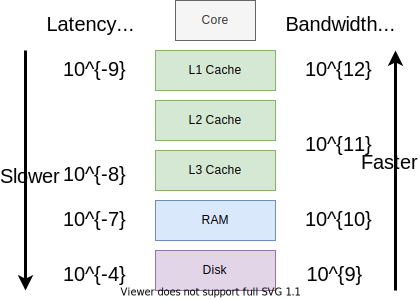
\includegraphics[width=1\textwidth]{figures/cachesketch.png}
      \end{center}
    \end{column}
  \end{columns}
  \vspace{\baselineskip}
  Optimisation: refactor algorithms to keep data in fast
  memory.

  {\footnotesize
    Check
    \href{https://colin-scott.github.io/personal_website/research/interactive_latency.html}{Colin
      Scott's page}
    for more detail on latencies.}
\end{frame}

\begin{frame}
  \frametitle{Cache memory: overview}

  \begin{exampleblock}{Features}
    \begin{itemize}[itemsep=6pt]
    \item Hierarchy of small, fast memory.
    \item Keep a copy of \emph{frequently used} data for faster access
    \end{itemize}
  \end{exampleblock}

  \pause

  \begin{challenge}{Issues}
    \begin{itemize}[itemsep=6pt]
    \item Frequently accessed data not known \emph{a priori}
    \item Only heuristics are possible $\Rightarrow$ \emph{princple of locality}
    \end{itemize}
  \end{challenge}

\end{frame}

\begin{frame}
  \frametitle{Principle of locality}
  \begin{itemize}
  \item Frequently accessed data often unknown before execution
  \item In practice, most programs exhibit \emph{locality} of data
    access.
  \item Optimised algorithms attempt to \emph{exploit} this
    locality.
  \end{itemize}

  \pause

  \begin{block}{Temporal locality}
    If I access data at some memory address, it is likely that I will
    do so again ``soon''.
  \end{block}

  \vskip -2pt

  \begin{block}{Spatial locality}
    If I access data at some memory address, it is likely that I will
    access neighbouring addresses.
  \end{block}
\end{frame}

\begin{frame}
  \frametitle{Temporal locality}

  On \structure{first access} to a new address, the data is:\\[-13pt]
  \begin{itemize}[itemsep=6pt]
  \item loaded from main memory to registers
  \item stored in cache
  \end{itemize}

  \vskip 20pt
  \pause

  \structure{Trade-off} solution:\\[-13pt]
  \begin{itemize}[itemsep=6pt]
  \item Small performance penalty for first access (storing is not free)
  \item Subsequent accesses use cached copy and are much faster.
  \end{itemize}
\end{frame}

\begin{frame}[fragile]
  \frametitle{Spatial locality}
  On \structure{first access} to a new address, the data is:\\[-13pt]
  \begin{itemize}[itemsep=6pt]
  \item loaded from main memory to registers
  \item stored in cache
  \item neighbouring addressed are also stored in cache
  \end{itemize}

  \vskip 20pt
  \pause

  \structure{Trade-off} solution:\\[-13pt]
  \begin{itemize}[itemsep=6pt]
  \item Large performance penalty for first access
  \item Subsequent accesses to neighbouring data will be fast
  \end{itemize}

\end{frame}

\begin{frame}[fragile]
  \frametitle{Example: sum reduction}
\begin{minted}{c}
                  float s[16] = 0
                  for (i = 0; i < N; i++)
                      s[i%16] += a[i];
\end{minted}

  \vskip 15pt

  \begin{itemize}[itemsep=6pt]
  \item Temporal locality
    \begin{itemize}[itemsep=4pt]
    \item 16 entries of \texttt{s} are accessed repeatedly
    \item Makes to keep all of \texttt{s} in cache
    \end{itemize}
  \item Spatial locality
    \begin{itemize}[itemsep=4pt]
    \item Contiguous entries of \texttt{a} are accessed
    \item When loading \texttt{a[i]} it makes sense to load \texttt{a[i+1]} too.
    \end{itemize}
  \end{itemize}
\end{frame}

\begin{frame}
  \frametitle{Designing a cache}
  \begin{block}{Important questions}
    \begin{enumerate}[itemsep=6pt]
    \item When we load data into the cache, where do we put it?
    \item If we have an address, how do determine if it is in the
      cache?
    \item What do we do when the cache becomes full?
    \end{enumerate}
  \end{block}

  \vskip 11pt

  \begin{itemize}[itemsep=4pt]
  \item Each datum uniquely referenced by its $K$-bit \emph{address}
  \item Need to turn this large memory address into a cache location
  \item $K$ is typically large ($\mathsf{2^{32}/2^{64}}$ addresses)
  \end{itemize}
\end{frame}

\begin{frame}
  \frametitle{Direct mapped cache}
  \begin{itemize}[itemsep=7pt]
  \item Cache can store $\mathsf 2^N$ bytes
  \item Divided into \emph{blocks} (or \emph{cache lines}) each of $\mathsf 2^M$ bytes
  \item Each address references one byte
  \item Use $N$ bits of address to select which slot
    in the cache to use
  \end{itemize}

  \vskip 11pt

  \structure{Simplest solution:} injection from RAM to cache
\end{frame}

\begin{frame}[fragile]
  \frametitle{Direct mapped caches: indexing}
  \begin{center}
    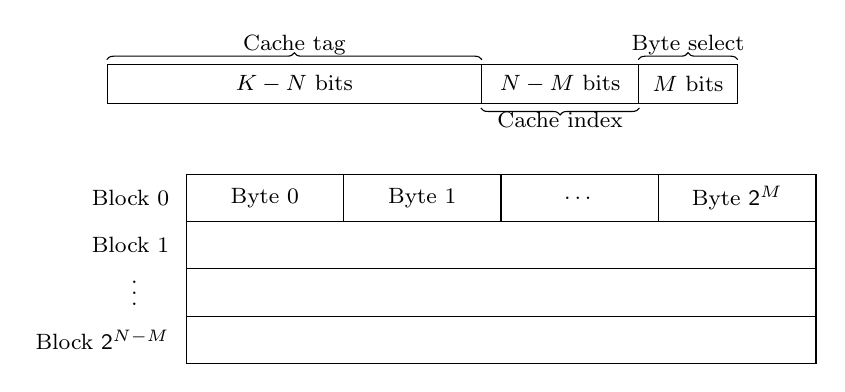
\begin{tikzpicture}
      \footnotesize \node[fit={(-1,1.5) (3.75, 2)}, inner sep=0pt,draw] (tag)
      {}; \node at (tag.center) {$K - N$ bits};
      \draw[decoration={brace,raise=0.05cm},decorate] (tag.north west) --
      (tag.north east) node [pos=0.5, anchor=south] {Cache tag};

      \node[fit={(3.75,1.5) (5.75, 2)}, inner sep=0pt,draw] (index) {}; \node at
      (index.center) {$N-M$ bits};
      \draw[decoration={brace,raise=0.05cm},decorate] (index.south east) --
      (index.south west) node[pos=0.5, anchor=north] {Cache index};

      \node[fit={(5.75,1.5) (7, 2)}, inner sep=0pt,draw] (select) {}; \node at
      (select.center) {$M$ bits}; \draw[decoration={brace,
        raise=0.05cm},decorate] (select.north west) -- (select.north east) node
      [pos=0.5, anchor=south] {Byte select};


      \node[fit={(0,0) (2,0.6)}, inner sep=0pt,draw] (byte0) {}; \node at
      (byte0.center) {Byte 0}; \node[fit={(2,0) (4,0.6)}, inner sep=0pt,draw]
      (byte1) {}; \node at (byte1.center) {Byte 1}; \node[fit={(4,0) (6,0.6)},
      inner sep=0pt,draw] (byte2) {}; \node at (byte2.center) {\dots};
      \node[fit={(6,0) (8,0.6)}, inner sep=0pt,draw] (byteM) {}; \node at
      (byteM.center) {Byte $\mathsf 2^M$};

      \node[left=0.1cm of byte0] {Block 0}; \node[fit={(0, 0) (8, -0.6)}, inner
      sep=0pt,draw] (block1) {}; \node[left=0.1cm of block1] {Block 1};
      \node[fit={(0, -0.6) (8, -1.2)}, inner sep=0pt,draw] (block2) {};
      \node[left=0.5cm of block2,yshift=0.1cm] {\vdots}; \node[fit={(0, -1.2)
        (8, -1.8)}, inner sep=0pt,draw] (blockN) {}; \node[left=0.1cm of blockN]
      {Block $\mathsf 2^{N-M}$};
    \end{tikzpicture}
  \end{center}
  \begin{itemize}
  \item \structure{Byte select}: Use lowest $M$ bits to select correct byte in block.
  \item \structure{Cache index}: Use next $N-M$ bits to select correct block.
  \item \structure{Cache tag}: Use remaining $K - N$ bits as a key.
  \end{itemize}
\end{frame}

\begin{frame}
  \frametitle{Choice of cache line size}
  \begin{itemize}[itemsep=8pt]
  \item Data is loaded one \emph{cache line} at a time
  \item Immediately exploits \emph{spatial locality}
  \item Larger cache lines are not always better
  \item Almost all modern CPUs use 64-byte size
  \end{itemize}

  \vskip 16pt

  \begin{block}{Rule of thumb}
    Cache-friendly algorithms work on cache line-sized chunks of data.
  \end{block}
\end{frame}

\begin{frame}[fragile]
  \frametitle{Direct mapped caches: eviction}
  \begin{itemize}[itemsep=4pt]
  \item \structure{Conflict:} two addresses have the same low bit pattern
  \item \structure{Resolution:} newest loaded address wins.
  \item This is a \emph{least recently used} (LRU) eviction policy.
  \end{itemize}

  \pause

  \begin{block}{What can go wrong?}
    \begin{columns}
      \begin{column}{0.45\textwidth}
\begin{minted}[fontsize=\small]{c}
int a[64], b[64], r = 0;
for (int i = 0; i < 100; i++)
   for (int j = 0; j < 64; j++)
       r += a[j] + b[j];
\end{minted}
      \end{column}
      \begin{column}{0.45\textwidth}
        \begin{itemize}
        \item 1KB cache
        \item 32-byte block size
        \item So $\mathsf{N=10, M=5}$
        \item 32 blocks in the cache
        \end{itemize}
      \end{column}
    \end{columns}
  \end{block}
\end{frame}

\newcommand{\myphantom}{\phantom{$a_{\mathsf{11:11}}$}}
\newcommand{\myvphantom}{\vphantom{$b_{\mathsf{11:11}}$}}
\newcommand{\myhphantom}{\vphantom{$a_{\mathsf{11:11}}$}}

\begin{frame}[fragile]
  \frametitle{Conflicts reduce \emph{effective} cache size}
  \begin{columns}
    \begin{column}{0.33\linewidth}
      \centering
\begin{minted}[fontsize=\footnotesize]{c}
for (int j = 0; j < 64; j++)
    r += a[j] + b[j];
\end{minted}

      \vskip 7pt
      \small
      \begin{onlyenv}<1>
        
\begin{tikzpicture} [nodes in empty cells, nodes={minimum
            width=1.4cm, minimum height=0.7cm, inner sep=0}, row sep=-\pgflinewidth,
          column sep=-\pgflinewidth]
          border/.style={draw} \matrix(matrix)[matrix of nodes,
          nodes={draw}] {
            \myphantom&\myphantom&\myphantom&\myphantom\\
            \myphantom&\myphantom&\myphantom&\myphantom\\
            \myphantom&\myphantom&\myphantom&\myphantom\\
            \myphantom&\myphantom&\myphantom&\myphantom\\
            \myphantom&\myphantom&\myphantom&\myphantom\\
            \myphantom&\myphantom&\myphantom&\myphantom\\
            \myphantom&\myphantom&\myphantom&\myphantom\\
            \myphantom&\myphantom&\myphantom&\myphantom\\
          };
        \end{tikzpicture}
      \end{onlyenv}%
      \begin{onlyenv}<2>
        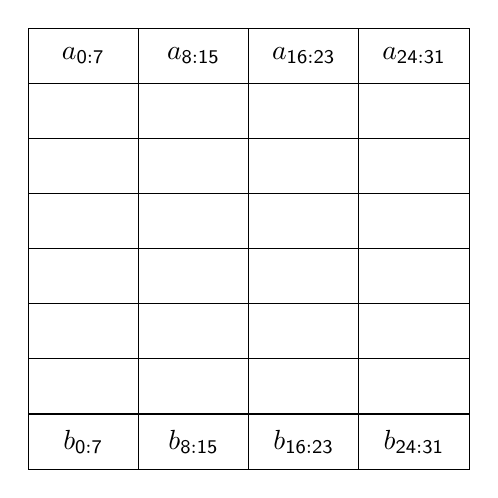
\begin{tikzpicture} [nodes in empty cells, nodes={minimum
            width=1.4cm, minimum height=0.7cm, inner sep=0}, row
          sep=-\pgflinewidth, column sep=-\pgflinewidth]
          border/.style={draw} \matrix(matrix)[matrix of nodes,
          nodes={draw}] {
            \myvphantom{}$a_{\mathsf{0:7}}$ & \myvphantom{}$a_{\mathsf{8:15}}$ &\myvphantom{}$a_{\mathsf{16:23}}$ & \myvphantom{}$a_{\mathsf{24:31}}$ \\
            \myphantom&\myphantom&\myphantom&\myphantom\\
            \myphantom&\myphantom&\myphantom&\myphantom\\
            \myphantom&\myphantom&\myphantom&\myphantom\\
            \myphantom&\myphantom&\myphantom&\myphantom\\
            \myphantom&\myphantom&\myphantom&\myphantom\\
            \myphantom&\myphantom&\myphantom&\myphantom\\
            $b_{\mathsf{0:7}}$ & $b_{\mathsf{8:15}}$ & $b_{\mathsf{16:23}}$ & $b_{\mathsf{24:31}}$ \\
          };
        \end{tikzpicture}
      \end{onlyenv}%
      \begin{onlyenv}<3>
        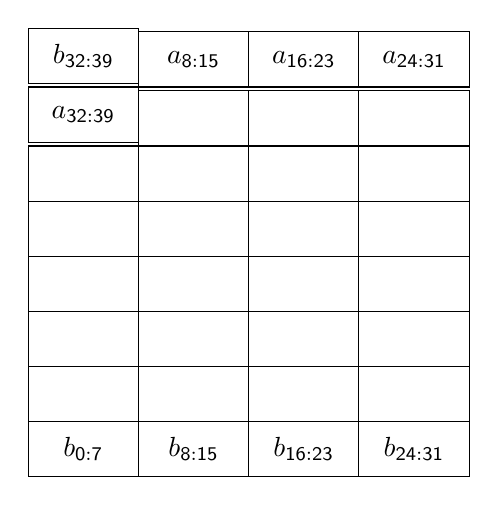
\begin{tikzpicture} [nodes in empty cells, nodes={minimum
            width=1.4cm, minimum height=0.7cm, inner sep=0}, row
          sep=-\pgflinewidth, column sep=-\pgflinewidth]
          border/.style={draw} \matrix(matrix)[matrix of nodes,
          nodes={draw}] {
            $b_{\mathsf{32:39}}$ & \myvphantom{}$a_{\mathsf{8:15}}$ & \myvphantom{}$a_{\mathsf{16:23}}$ & \myvphantom{}$a_{\mathsf{24:31}}$ \\
            $a_{\mathsf{32:39}}$&\myhphantom&\myhphantom&\myhphantom\\
            \myphantom&\myphantom&\myphantom&\myphantom\\
            \myphantom&\myphantom&\myphantom&\myphantom\\
            \myphantom&\myphantom&\myphantom&\myphantom\\
            \myphantom&\myphantom&\myphantom&\myphantom\\
            \myphantom&\myphantom&\myphantom&\myphantom\\
            $b_{\mathsf{0:7}}$   & $b_{\mathsf{8:15}}$ & $b_{\mathsf{16:23}}$ & $b_{\mathsf{24:31}}$ \\
          };
        \end{tikzpicture}
      \end{onlyenv}%
      \begin{onlyenv}<4>
        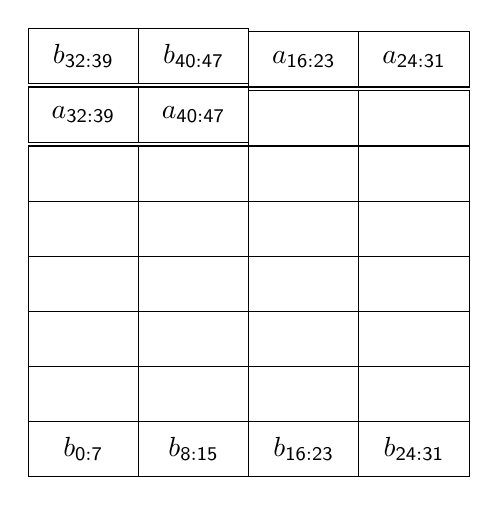
\begin{tikzpicture} [nodes in empty cells, nodes={minimum
            width=1.4cm, minimum height=0.7cm, inner sep=0}, row
          sep=-\pgflinewidth, column sep=-\pgflinewidth]
          border/.style={draw} \matrix(matrix)[matrix of nodes,
          nodes={draw}] {
            $b_{\mathsf{32:39}}$ & $b_{\mathsf{40:47}}$  & \myvphantom{}$a_{\mathsf{16:23}}$ & \myvphantom{}$a_{\mathsf{24:31}}$ \\
            $a_{\mathsf{32:39}}$ & $a_{\mathsf{40:47}}$ &\myhphantom&\myhphantom\\
            \myphantom&\myphantom&\myphantom&\myphantom\\
            \myphantom&\myphantom&\myphantom&\myphantom\\
            \myphantom&\myphantom&\myphantom&\myphantom\\
            \myphantom&\myphantom&\myphantom&\myphantom\\
            \myphantom&\myphantom&\myphantom&\myphantom\\
            $b_{\mathsf{0:7}}$   & $b_{\mathsf{8:15}}$  & $b_{\mathsf{16:23}}$ & $b_{\mathsf{24:31}}$ \\
          };
        \end{tikzpicture}
      \end{onlyenv}%
      \begin{onlyenv}<5>
        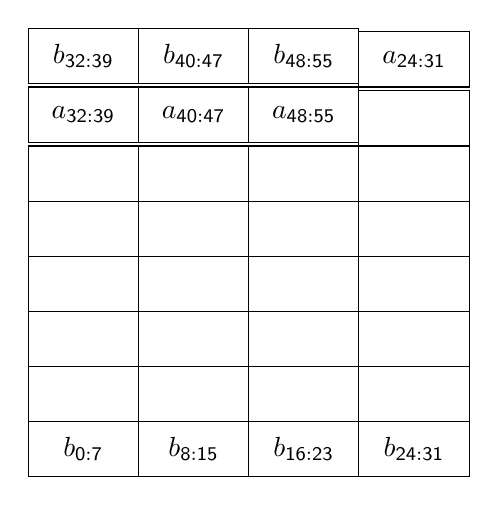
\begin{tikzpicture} [nodes in empty cells, nodes={minimum
            width=1.4cm, minimum height=0.7cm, inner sep=0}, row
          sep=-\pgflinewidth, column sep=-\pgflinewidth]
          border/.style={draw} \matrix(matrix)[matrix of nodes,
          nodes={draw}] {
            $b_{\mathsf{32:39}}$ & $b_{\mathsf{40:47}}$ & $b_{\mathsf{48:55}}$ & \myvphantom{}$a_{\mathsf{24:31}}$ \\
            $a_{\mathsf{32:39}}$ & $a_{\mathsf{40:47}}$ & $a_{\mathsf{48:55}}$ &
            \myhphantom{}\\
            &             &             &             \\
            &             &             &             \\
            &             &             &             \\
            &             &             &             \\
            &             &             &             \\
            $b_{\mathsf{0:7}}$   & $b_{\mathsf{8:15}}$  & $b_{\mathsf{16:23}}$ & $b_{\mathsf{24:31}}$ \\
          };
        \end{tikzpicture}
      \end{onlyenv}%
      \begin{onlyenv}<6->
        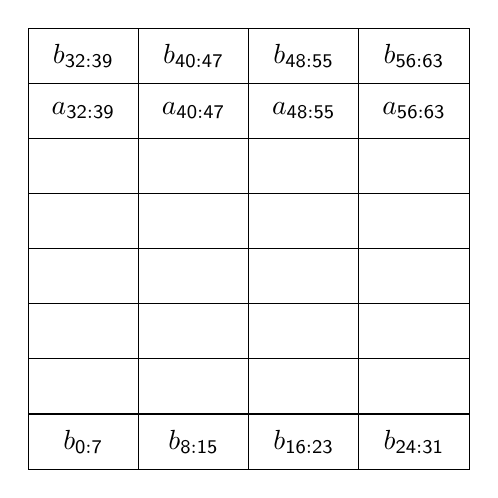
\begin{tikzpicture} [nodes in empty cells, nodes={minimum
            width=1.4cm, minimum height=0.7cm, inner sep=0}, row
          sep=-\pgflinewidth, column sep=-\pgflinewidth]
          border/.style={draw} \matrix(matrix)[matrix of nodes,
          nodes={draw}] {
            $b_{\mathsf{32:39}}$ & $b_{\mathsf{40:47}}$ & $b_{\mathsf{48:55}}$ & $b_{\mathsf{56:63}}$ \\
            $a_{\mathsf{32:39}}$ & $a_{\mathsf{40:47}}$ & $a_{\mathsf{48:55}}$ & $a_{\mathsf{56:63}}$ \\
            &             &             &             \\
            &             &             &             \\
            &             &             &             \\
            &             &             &             \\
            &             &             &             \\
            $b_{\mathsf{0:7}}$   & $b_{\mathsf{8:15}}$  & $b_{\mathsf{16:23}}$ & $b_{\mathsf{24:31}}$ \\
          };
        \end{tikzpicture}
      \end{onlyenv}%
    \end{column}
    \begin{column}{0.45\linewidth}
\begin{minted}[fontsize=\scriptsize]{c}
&a[00] = ... 00000 00000 => block  0, byte offset 0
&a[01] = ... 00000 00100 => block  0, byte offset 4
&a[02] = ... 00000 01000 => block  0, byte offset 8
&a[03] = ... 00000 01100 => block  0, byte offset 12
&a[04] = ... 00000 10000 => block  0, byte offset 16
&a[05] = ... 00000 10100 => block  0, byte offset 20
&a[06] = ... 00000 11000 => block  0, byte offset 24
&a[07] = ... 00000 11100 => block  0, byte offset 28
...
&b[00] = ... 11100 00000 => block 28, byte offset 0
&b[01] = ... 11100 00100 => block 28, byte offset 4
&b[02] = ... 11100 01000 => block 28, byte offset 8
&b[03] = ... 11100 01100 => block 28, byte offset 12
&b[04] = ... 11100 10000 => block 28, byte offset 16
&b[05] = ... 11100 10100 => block 28, byte offset 20
&b[06] = ... 11100 11000 => block 28, byte offset 24
&b[07] = ... 11100 11100 => block 28, byte offset 28
...
\end{minted}
    \end{column}
  \end{columns}
\end{frame}
\begin{frame}[fragile]
  \frametitle{Cache thrashing}
  \begin{block}{What can go wrong?}
    \begin{columns}
      \begin{column}{0.45\textwidth}
\begin{minted}[fontsize=\scriptsize]{c}
int A[64], B[64], r = 0;
for (int i = 0; i < 100; i++)
   for (int j = 0; j < 64; j++)
       r += A[j] + B[j];
\end{minted}
      \end{column}
      \begin{column}{0.45\textwidth}
        \begin{itemize}
        \item 1KB cache
        \item 32 byte block size
        \item So $N=10$, $M=5$. \\32 blocks in the cache.
        \end{itemize}
      \end{column}
    \end{columns}
  \end{block}


  \begin{itemize}[wide=0pt,itemsep=4pt]
  \item We need $\mathsf{2 \cdot 64 \cdot 4 = 512}$ bytes to store $A$ and $B$
    in cache.
  \item This only requires 16 blocks, so our cache is large enough.
  \item If low bits of addresses match, same cache lines are mapped.
  \item In the worst case, every load of \texttt{B[j]} evicts
    \texttt{A[j]}, and vice versa.
  \end{itemize}

\end{frame}

\begin{frame}[t]
  \frametitle{Cache associativity}
  \begin{itemize}[itemsep=8pt]
  \item Direct mapped
    \begin{itemize}[wide=0pt,itemsep=6pt]
    \item Each RAM \emph{block} maps to exactly one cache
      line.
    \item LRU eviction policy (new data overwrite old)
    \end{itemize}
  \item<2> Fully associative
    \begin{itemize}[wide=0pt,itemsep=6pt]
    \item Each RAM \emph{byte} can map to any cache line
    \item Data is stored in first unused cache line
    \item If all lines are used, overall LRU one is replaced
    \item Most flexible, but also mostexpensive
    \end{itemize}
  \end{itemize}
\end{frame}

\begin{frame}
  \frametitle{$k$-way set associative cache}
  \begin{itemize}[itemsep=8pt]
  \item $k$ ``copies'' of a direct mapped cache.
  \item Each block from main memory maps to $k$ cache lines, called \emph{sets}.
  \item Typically use LRU eviction.
  \item Usual choice: $N \in \{2, 4, 8, 16\}$.
  \item Skylake has $N = 8$ for L1, $N = 16$ for L2, $N = 11$
    for L3.
  \end{itemize}
\end{frame}

\begin{frame}
  \frametitle{Exercises 2/3: memory bandwidth/saturation}
  \begin{enumerate}[itemsep=8pt]
  \item Split into small groups
  \item Make sure one person per group has access to Hamilton
  \item Benchmark memory bandwidth as a function of vector size
  \item You can use the bash script from last week.
  \item Ask questions!
  \end{enumerate}
\end{frame}

\begin{frame}
  \frametitle{Exercise 2: results}
  \pgfplotsset{
    execute at begin axis={
      \pgfplotsset{
        width=.8\textwidth,
        height=.8\textheight,
      }
    }
  }
  \begin{center}
    \begin{tikzpicture}
      \begin{axis}[xlabel={Bytes},
        ylabel near ticks,
        axis y line*=left,
        ylabel={MB/s},
        xlabel={Array size},
        xmode=log,
        xtick={1,16,256,4096,65536,1048576},
        xticklabels={1kB,16kB,256kB,4MB,64MB,1GB},
        log basis x={10},
        legend style={
          cells={
            anchor=west,
            align=left},
          fill=bgcolor},]
        \pgfplotstableread[row sep=\\]{%
          Bytes clcopy clload clstore\\
          1 139083.51 179357.99 134508.89\\
          2 196557.66 200900.73 170423.91\\
          4 283864.91 276420.73 190769.38\\
          8 343844.98 325363.41 201581.34\\
          16 382052.17 360816.24 207229.80\\
          32 381795.36 324163.59 193009.02\\
          64 104430.65 104115.72 104094.22\\
          128 105418.11 105274.71 105298.06\\
          256 105805.33 105618.95 105592.56\\
          512 96180.42 94651.42 101184.04\\
          1024 81360.92 79856.34 95944.93\\
          2048 79612.24 78885.03 95593.15\\
          4096 79301.66 83244.18 86619.98\\
          8192 80204.31 92788.95 84685.91\\
          16384 51740.62 60992.59 46804.81\\
          32768 17590.26 16579.85 12563.31\\
          65536 18087.89 16594.21 12543.57\\
          131072 18173.68 16583.02 12661.70\\
          262144 17887.64 16706.78 12663.04\\
          524288 17873.13 16706.51 12651.07\\
          1048576 18037.20 16718.25 12612.07\\
        }\mydata
        \addplot [JungleGreen, very thick, mark=*, mark size=2.5pt]
        table[x=Bytes,y=clcopy] {\mydata};\label{clcopy}
        \addlegendentry{\texttt{clcopy}}

        \addplot [MidnightBlue, very thick, mark=diamond, mark size=2.5pt]
        table[x=Bytes,y=clload] {\mydata};\label{clload}
        \addlegendentry{\texttt{clload}}

        \addplot [Purple, very thick, mark=triangle, mark size=2.5pt]
        table[x=Bytes,y=clstore] {\mydata};\label{clstore}
        \addlegendentry{\texttt{clstore}}

        \only<2>{%
          \addlegendimage{/pgfplots/refstyle=sum-sp-avx}
          \addlegendentry{\texttt{sum\_sp\_avx}}
        }

      \end{axis}
      \pause
      \begin{axis}[xlabel={},
        ylabel near ticks,
        axis y line*=right,
        ylabel={MFlops/s},
        xmode=log,
        xticklabels={},
        log basis x={2},
        legend pos={outer north east},
        legend style={cells={anchor=west, align=left}},]
        \pgfplotstableread[row sep=\\]{%
          Bytes scalar avx\\
          1 4721.23 25633.48\\
          2 4566.17 35462.91\\
          4 4497.61 40717.13\\
          8 4465.51 37820.79\\
          16 4443.53 36595.48\\
          32 4424.07 33791.29\\
          64 4222.61 25780.94\\
          128 4258.17 26158.12\\
          256 4204.51 26281.52\\
          512 4384.87 23034.10\\
          1024 4394.45 18759.08\\
          2048 4386.30 18655.37\\
          4096 4396.57 18868.36\\
          8192 4398.89 18856.77\\
          16384 4084.19 13711.12\\
          32768 3387.52 5583.20\\
          65536 3399.47 5633.13\\
          131072 3412.19 5582.03\\
          262144 3399.07 5573.66\\
          524288 3404.33 5581.31\\
          1048576 3428.27 5645.72\\
        }\mydata

        % \addlegendimage{/pgfplots/refstyle=clcopy}
        % \addlegendentry{\texttt{clcopy}}
        % \addlegendimage{/pgfplots/refstyle=clload}
        % \addlegendentry{\texttt{clload}}
        % \addlegendimage{/pgfplots/refstyle=clstore}
        % \addlegendentry{\texttt{clstore}}

        \addplot [Black, very thick, mark=o, mark size=2.5pt] table[x=Bytes,y=avx] {\mydata}; \label{sum-sp-avx}
        % \addlegendentry{test};
      \end{axis}
    \end{tikzpicture}
  \end{center}
\end{frame}


\begin{frame}
  \frametitle{Interpretation}
  \small
  \begin{itemize}
   % 35 Gflop/s is the single-core Flop rate
  \item Vectorised addition requires 1 32Byte load/cycle (for the 8
    floats)
  \item Accumulation parameter held in a register.
  \item[$\Rightarrow$] requires sustained load bandwidth of $4 \cdot 35 = 148$GB/s

    % Sustained bandwidth: look at the clload benchmark in the graph.
    % B/Flop: divide BW by Flop rate of machine (35GFlop/s) and multiply by 8.
    % float/Flop: divide B/Flop by number of bytes in float.
    % peak: divide the (float/Flop / 8) by Flop rate.
  \item From L1 (less than 32kB) we see sustained bandwidth of around
    370GB/s or 90B/Flop $\Rightarrow$ 22 float/Flop  $\Rightarrow$
    floating-point throughput is limit.

  \item L2 (less than 512kB) provides around 100GB/s or around
    25B/Flop $\Rightarrow$ 6.25 floats/Flop $\Rightarrow$ peak
    is around 27GFlop/s.

  \item L3 (less than 16MB) provides around 78GB/s or around
    18B/Flop $\Rightarrow$ 4.45 floats/cycle $\Rightarrow$ peak
    is around 19GFlop/s.

  \item Main memory provides around 17.5GB/s or around 4B/Flop
    $\Rightarrow$ 1float/cycle $\Rightarrow$ peak is around 4.5GFlop/s.

  \end{itemize}
\end{frame}

\begin{frame}
  \frametitle{AVX throughput with bandwidth-induced limits}
  \begin{center}
    \pgfplotsset{
      execute at begin axis={
        \pgfplotsset{
          width=0.8\textwidth,
          height=.8\textheight,
        }
      }
    }
    \begin{tikzpicture}
      \begin{axis}[xlabel={},
        ylabel near ticks,
        ylabel={MFlops/s},
        xmode=log,
        xticklabels={},
        log basis x={2},
        legend pos={north east},
        legend style={cells={anchor=west, align=left},
          fill=bgcolor},]
        \pgfplotstableread[row sep=\\]{%
          Bytes scalar avx\\
          1 4721.23 25633.48\\
          2 4566.17 35462.91\\
          4 4497.61 40717.13\\
          8 4465.51 37820.79\\
          16 4443.53 36595.48\\
          32 4424.07 33791.29\\
          64 4222.61 25780.94\\
          128 4258.17 26158.12\\
          256 4204.51 26281.52\\
          512 4384.87 23034.10\\
          1024 4394.45 18759.08\\
          2048 4386.30 18655.37\\
          4096 4396.57 18868.36\\
          8192 4398.89 18856.77\\
          16384 4084.19 13711.12\\
          32768 3387.52 5583.20\\
          65536 3399.47 5633.13\\
          131072 3412.19 5582.03\\
          262144 3399.07 5573.66\\
          524288 3404.33 5581.31\\
          1048576 3428.27 5645.72\\
        }\mydata

        \addplot [Black, very thick, mark=o, mark size=2.5pt]
        table[x=Bytes,y=avx] {\mydata}; \label{sum-sp-avx}
        \addlegendentry {\texttt{sp\_sum\_avx}};

        \addplot[draw=MidnightBlue, mark=none, very thick] coordinates
        {(1,37 * 1024)(1048576,37 * 1024)};
        \addlegendentry {L1 peak}

        \addplot[draw=Green, densely dashed, mark=none, very thick] coordinates
        {(1,27 * 1024)(1048576,27 * 1024)};
        \addlegendentry {L2 peak}

        \addplot[draw=Plum, loosely dashed, mark=none, very thick] coordinates
        {(1,19 * 1024)(1048576,19 * 1024)};
        \addlegendentry {L3 peak}

        \addplot[draw=BrickRed, densely dotted, mark=none, very thick] coordinates
        {(1,4.5 * 1024)(1048576,4.5 * 1024)};
        \addlegendentry {RAM peak}

        % \addlegendentry{test};
      \end{axis}

    \end{tikzpicture}
  \end{center}
\end{frame}

\begin{frame}
  \frametitle{Memory/node topology}
  \texttt{likwid-topology} reports an ASCII version of diagrams like
  this.
  \begin{center}
    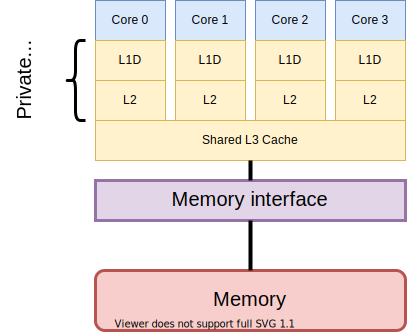
\includegraphics[height=0.5\textheight]{figures/cacheschematic.png}
  \end{center}
\end{frame}

\begin{frame}
  \frametitle{Exercise 3: results}
  \begin{center}
    \begin{tikzpicture}
      \begin{groupplot}[
        group style={
          group size=2 by 2,
          ylabels at=edge left,
          vertical sep=30,
        },
        width=0.5\textwidth,
        height=0.5\textheight,
        % ytick align=outside,
        % xtick align=outside,
        enlarge x limits=false,
        every axis plot/.append style={
          mark repeat = 8,
          mark phase = 7,
          very thick}]
        \pgfplotstableread[row sep=\\]{
          n_cores L1_BW_s L1_BW_d L2_BW_s L2_BW_d L3_BW_s L3_BW_d RAM_BW_s RAM_BW_d\\
          1 359562.59 718325.90 102548.42 207833.69 93467.75 157614.11 16687.80 33120.53 \\
          2 721829.27 1429180.86 207031.98 420537.99 89590.96 174879.97 31107.62 62106.37 \\
          3 1082831.84 2150035.43 316615.14 632355.47 36855.37 73808.74 37067.04 72820.11 \\
          4 1432279.97 2865225.02 422934.97 822507.06 36084.42 70965.95 37197.00 72338.65 \\
          5 1794707.96 3577290.04 527886.48 1036161.08 46562.16 91787.63 36830.54 72697.84 \\
          6 2148941.26 4296591.91 614862.70 1242796.55 53297.72 105876.73 36740.37 72598.77 \\
          7 2499524.85 4984735.09 688215.47 1381141.42 37210.03 75402.40 36105.43 71570.32 \\
          8 2867379.26 5716318.40 822500.98 1643788.99 35728.12 70658.99 35645.25 70677.07 \\
          9 3210180.71 6436142.31 920771.08 1809591.57 40395.21 79698.98 37777.93 75056.80 \\
          10 3561580.49 7144034.38 1056340.22 1987139.50 44509.07 88732.89 38548.73 77075.25 \\
          11 3943073.21 7881467.34 1140581.07 2258960.09 40507.61 81971.73 39697.55 79043.85 \\
          12 4277067.08 8565095.31 1232360.62 2364065.23 40693.37 81595.04 40556.29 80846.18 \\
          13 4654549.90 9272633.68 1344272.57 2647167.30 44068.54 87853.04 41205.32 82380.80 \\
          14 4982662.27 9334888.12 1392644.41 2779309.87 47173.54 93935.62 42001.39 83814.07 \\
          15 5360826.21 9986699.13 1544473.06 3027750.63 50037.20 99986.79 42376.67 84763.93 \\
          16 5713086.62 10711024.40 1522086.75 3220381.49 42834.39 86674.05 42626.62 85247.02 \\
          17 6072311.87 10299622.36 1611954.55 3375179.84 45385.87 91347.43 45286.52 90423.60 \\
          18 6044085.81 12833506.11 1779469.17 3539726.86 48554.12 96802.33 47902.17 95802.80 \\
          19 6786741.61 13539967.66 1850540.03 3687733.08 51356.84 102265.69 50585.07 101037.01 \\
          20 7137930.08 13317785.27 2006238.60 3805763.39 53463.35 106733.71 53201.67 106371.40 \\
          21 7482809.77 13847550.54 2098588.90 4068744.74 56562.46 112568.89 55835.99 111687.58 \\
          22 7878046.81 13806374.41 2165347.05 4222468.80 58690.18 118114.10 58473.36 117037.47 \\
          23 8221806.00 15382207.64 2221649.03 4344435.74 61710.96 123718.10 61122.06 122156.66 \\
          24 7927579.16 15665984.24 2321709.02 4477167.49 64776.72 128197.90 63830.76 127453.84 \\
          25 8150306.47 16365605.80 2315787.00 4562515.75 67261.60 135485.78 66422.08 132807.27 \\
          26 8829567.42 15884064.83 2408858.04 4780972.64 69836.39 139498.44 68941.80 137802.12 \\
          27 8685841.12 17117836.75 2387482.99 5018420.17 72363.98 144423.24 71578.17 143557.45 \\
          28 9544283.51 18147418.92 2525411.31 5340110.65 75301.76 149895.03 74230.16 148650.42 \\
          29 9400028.63 18666268.14 2516164.41 5326315.28 77958.64 156748.56 76958.81 153894.12 \\
          30 9554447.06 19298739.80 2790123.91 5354146.94 80915.69 159949.82 79692.34 158719.76 \\
          31 10433054.16 19621439.66 2941157.16 5758088.00 84086.18 164792.35 82245.24 164311.21 \\
          32 9517718.13 20004587.18 3009546.40 5789788.49 85934.83 169637.05 84594.32 164840.20 \\
          33 10232124.00 20574220.21 3100564.60 6100656.39 88275.57 176011.62 87569.57 174928.53 \\
          34 10068422.80 21482759.89 3200911.62 6260595.84 91124.70 180778.14 90223.02 180201.76 \\
          35 10249015.71 21964479.70 3182454.80 6305036.65 92879.62 187192.49 92948.85 185709.73 \\
          36 11157807.51 22113999.03 3233898.35 6583234.78 96050.88 190766.29 95508.47 190819.62 \\
          37 11591105.23 21740540.91 3278031.67 6428672.78 99088.80 195703.68 97909.95 195682.40 \\
          38 11039267.03 23185154.65 3292111.55 6588977.81 101625.02 202822.71 100731.91 201396.93 \\
          39 11987792.45 23619435.13 3420569.00 7089790.05 103842.29 208231.73 103298.10 206508.51 \\
          40 11522793.70 22984896.94 3624087.92 7030788.69 106062.21 214563.72 106065.87 211970.97 \\
          41 11721261.82 25105421.51 3636140.35 7282713.36 108789.90 218272.01 108815.48 217119.75 \\
          42 12509265.38 25507883.99 3868282.87 7316028.19 111740.30 223091.38 111370.32 222573.36 \\
          43 12977721.16 25895948.79 3791424.51 7759440.79 115332.26 228764.62 113951.09 227739.48 \\
          44 14117830.30 26428837.87 3930534.07 7838905.38 116966.94 234883.63 116487.91 232762.83 \\
          45 13448898.76 26873827.81 4002230.05 7756856.85 120330.12 239792.70  119050.38 237998.50 \\
          46 13684907.60 27559082.89 4055127.96 8131406.51 123025.13 244879.24 121790.47 243377.34 \\
          47 14834494.15 27915539.75 4086299.14 8178471.37 125405.83 250042.99 124287.49 248426.69 \\
          48 13367126.05 28167332.37 4169877.59 8089267.79 126428.62 256717.35 126813.23 253629.26 \\
          49 14357233.43 27460880.32 4279831.41 8168680.68 130750.63 259558.72 129593.51 259093.49 \\
          50 14554399.46 29084276.91 4272329.50 8398844.56 133311.72 266825.46 132279.64 264447.59 \\
          51 14705473.07 29416130.08 4399558.05 8448271.08 136846.81 269876.09 134829.09 269503.64 \\
          52 15001494.78 30202348.21 4381791.69 8429400.30 138586.95 277526.97 137456.42 274652.69 \\
          53 15108742.17 30067459.62 4330851.42 8499734.61 140856.64 280399.50 140055.96 279905.53 \\
          54 15280178.83 30800588.85 4546587.67 8962682.05 144014.53 285863.41 142624.32 284492.64 \\
          55 15449103.84 30844806.00 4412848.57 9044119.86 146941.72 289459.90 145205.98 290233.35 \\
          56 15625293.83 30897637.35 4441186.37 9104807.57 148281.27 296790.57 148152.55 295212.43 \\
          57 16029074.29 31660060.53 4607576.33 9081793.88 152655.63 303244.36 150227.64 300980.31 \\
          58 16012455.16 31866405.60 4551664.81 9282251.68 154382.28 310178.94 153026.34 305702.18 \\
          59 16663756.27 32390429.80 4615455.86 9423904.11 156691.45 315924.20 155265.89 310212.36 \\
          60 16419722.15 32395055.56 4836629.63 9392320.92 159487.23 319401.58 158090.11 315610.31 \\
          61 16511949.58 33463155.29 4803169.57 9648845.28 162249.72 323915.03 161049.94 321768.21 \\
          62 16553914.44 33295048.43 4828531.57 9380583.74 165465.24 331113.41 163558.58 327158.48 \\
          63 16965150.19 33754853.61 4881156.55 9691132.23 167305.89 336139.75 166134.11 332193.99 \\
          64 16983378.50 34119105.24 5038546.06 9846248.84 170155.84 338246.38 168490.54 336553.16 \\}\mydata

        \nextgroupplot[ticklabel style={font=\tiny},
        label style={font=\scriptsize},
        legend style={font=\scriptsize, fill=bgcolor},
        ylabel={MB/s}, legend pos={south east}]
        \addplot[Blue, dashed, mark=o, mark options=solid] table[x=n_cores, y=L1_BW_s] \mydata;
        \addlegendentry{L1 (1 socket)}
        \addplot[Red, mark=square,] table[x expr=\thisrowno{0}*2, y=L1_BW_d] \mydata;
        \addlegendentry{L1 (2 sockets)}

        \nextgroupplot[ticklabel style={font=\tiny},
        label style={font=\scriptsize},
        legend style={font=\scriptsize, fill=bgcolor},
        legend pos={south east}]
        \addplot[Blue, dashed, mark=o, mark options=solid] table[x=n_cores, y=L2_BW_s] \mydata;
        \addlegendentry{L2 (1 socket)}
        \addplot[Red, mark=square,] table[x expr=\thisrowno{0}*2, y=L2_BW_d] \mydata;
        \addlegendentry{L2 (2 sockets)}

        \nextgroupplot[ticklabel style={font=\tiny},
        label style={font=\scriptsize},
        xlabel style={yshift=1ex},
        legend style={font=\scriptsize, fill=bgcolor},
        ylabel={MB/s}, xlabel={Cores}, legend pos={south east}]
        \addplot[Blue, dashed, mark=o, mark options=solid] table[x=n_cores, y=L3_BW_s] \mydata;
        \addlegendentry{L3 (1 socket)}
        \addplot[Red, mark=square,] table[x expr=\thisrowno{0}*2, y=L3_BW_d] \mydata;
        \addlegendentry{L3 (2 sockets)}

        \nextgroupplot[ticklabel style={font=\tiny},
        label style={font=\scriptsize},
        legend style={font=\scriptsize, fill=bgcolor},
        xlabel style={yshift=1ex},
        xlabel={Cores}, legend pos={south east}]
        \addplot[Blue, dashed, mark=o, mark options=solid] table[x=n_cores, y=RAM_BW_s] {\mydata};
        \addlegendentry{RAM (1 socket)}
        \addplot[Red, mark=square,] table[x expr=\thisrowno{0}*2, y=RAM_BW_d] {\mydata};
        \addlegendentry{RAM (2 sockets)}
      \end{groupplot}
    \end{tikzpicture}
  \end{center}
\end{frame}

\begin{frame}
  \frametitle{Conclusions on hardware architecture}
  \structure{Performance considerations}
    \begin{itemize}[wide=0pt]
    \item How many instructions are required
    \item How efficiently a processor can execute those instructions
    \item The runtime contribution of the data transfers
    \end{itemize}
    \pause

  \structure{Complex ``topology'' of hardware}
    \begin{itemize}[wide=0pt]
    \item Many layers of parallelism in modern hardware
    \item Sockets: around 1-4 CPUs on a typical motherboard
    \item Cores: around 4-32 cores in a typical CPU
    \item Vectorisation: 2-16 \texttt{float}s per vector registers
    \item Superscalar execution: typically 2-8 instructions per cycle
    \end{itemize}
\end{frame}

\end{document}
